\section{The Infinite Range Ising Model}
\subsection{Motivation - Mean Field Theory}
The Hamiltonian of the infinite range Ising model is:
\begin{equation}
    H = - \frac{J}{N}\sum_{x, y}\sigma_x \sigma_y - B\sum_x \sigma_x
\end{equation}
The sum is taken over all pairs of spin, so every spin interacts with the same interaction strength as every other spin. This is obviously unrealistic physically, but it is of interest to study as the solution gives us insight into mean field theory, which is a approximation technique that can tell us a lot about second-order phase transitions.

Why is this? We can move the sum $\frac{1}{N}\sum_y$ inside of the $\sum_x$ summation, and then this looks like the spin $\sigma_x$ interacts with the mean/average spin $\frac{1}{N}\sum_y \sigma_y$ (this is analytically true for this model). Note that mean field theory is wrong in general (it is an approximation technique) but it is a widely used tool (e.g. in condensed matter theory).

\subsection{Gaussian Integral}
Recall from our teaser last time the identity:
\begin{equation}
    1 = \left(\frac{NJ}{\pi k_B T}\right)^{1/2}\int_{-\infty}^\infty d\phi e^{-\frac{NJ}{k_B T}\phi^2}
\end{equation}
How is this integral evaluated? This is a classic integral; let's go through it together. Let's consider the general (1-D) Gaussian integral:
\begin{equation}
    \int_{-\infty}^\infty dx e^{-ax^2}
\end{equation}
The trick is to write the above as a square root of its square:
\begin{equation}
    \int_{-\infty}^\infty dx e^{-ax^2} = \sqrt{\left( \int_{-\infty}^\infty dx e^{-ax^2}\right)^2} = \sqrt{\left( \int_{-\infty}^\infty dx e^{-ax^2}\right)\left(\int_{-\infty}^\infty dy e^{-ay^2}\right)}
\end{equation}
Now this looks like a 2-dimensional integral; one we can solve by going into polar coordinates!
\begin{equation}
    \int_{-\infty}^\infty dx e^{-ax^2} = \sqrt{\int_{-\infty}^\infty dxdy e^{-a(x^2 + y^2)}} = \sqrt{\int_{0}^{2\pi}d\phi \int_{0}^\infty rdr e^{-ar^2}}
\end{equation}
Now making the substitution $u = ar^2$, $du = 2ardr$, the integral is easily solved:
\begin{equation}
    \int_{-\infty}^\infty dx e^{-ax^2} = \sqrt{2\pi \frac{1}{2}\frac{1}{a}} = \sqrt{\frac{\pi}{a}}
\end{equation}
which is the familiar result.

\subsection{Solving the Infinite Range Ising Model}
Now, let us take this result, and consider that we can shift the variable of integration $\phi \to \phi + \sum_x \sigma_x$ (plus a constant - does not change the result of the integral as the range of integration is $-\infty$ to $\infty$):
\begin{equation}\label{eq-1convenientform}
    1 = \left(\frac{NJ}{\pi k_B T}\right)^{1/2}\int_{-\infty}^\infty d\phi e^{-\frac{NJ}{k_B T}\left(\phi - \frac{1}{N}\sum_x \sigma_x\right)^2}
\end{equation}
Now, recall back to the partition function for the model we wish to compute:
\begin{equation}
    Z[T, B, N] = \sum_{\text{spins}} e^{\frac{J}{Nk_B T}\sum{x, y}\sigma_x\sigma_y + \frac{B}{k_B T}\sum_x \sigma_x}
\end{equation}
Now let us insert a factor of $1$ as in Eq. \eqref{eq-1convenientform}; this will yield some useful cancellations:
\begin{equation}
    Z[T, B, N] = \left(\frac{NJ}{\pi k_B T}\right)^{1/2}\int_{-\infty}^\infty d\phi e^{-\frac{NJ}{k_B T}\phi^2}\sum_{\text{spins}} e^{\frac{B + 2J\phi}{k_B T}\sum_x\sigma_x}
\end{equation}
Now, the sum over spins can be carried out explicitly as we can just independently sum over and take the product:
\begin{equation}
    \sum_{\text{spins}} e^{\frac{B + 2J\phi}{k_B T}\sum_x\sigma_x} = \left(e^{\frac{B + 2J\phi}{k_B T}} + e^{-\frac{B + 2J\phi}{k_B T}}\right)^N
\end{equation}
Recognizing the identity $e^{x} + e^{-x} = 2\cosh(x)$, our partition function becomes:
\begin{equation}
    Z[T, B, N] = \left(\frac{NJ}{\pi k_B T}\right)^{1/2} \int_{-\infty}^\infty d\phi e^{-N\left[\frac{J}{k_B T}\phi^2 - \ln(2\cosh(\frac{B + 2J\phi}{k_B T}))\right]}
\end{equation}
So we are left with an integral that is hard. What do we do? Remember that we are doing stat mech/thermo here, so $N \to \infty$. In this case, we can evaluate this integral by the saddle point technique. We replace the integral with where the integrand is maximized\footnote{Note: we are allowed to search in the complex plane; more formally, we have an integral over the real line, the contour which we then deform off the real axis such that the contour follows the ``mountain passes'' in the complex landscape. Here this is not so complicated, as we have real solutions.}:
\begin{equation}
    Z[T, B, N] \approx e^{-N\inf_\phi\left[\frac{J}{k_B T}\phi^2 - \ln(\cosh(\frac{B + 2J\phi}{k_B T}))\right] + N\ln 2}
\end{equation}
where $\inf$ (infimum) denotes the greatest lower bound. So then the Helmholtz free energy is:
\begin{equation}
    F[T, B, N] = k_B T N \inf_\phi \left(\frac{J\phi^2}{k_B T} - \ln\cosh\frac{B + 2J\phi}{k_B T}\right) - k_B T N\ln 2
\end{equation}
So, we should try to find this infimum/minimum; of course this is a calculus problem, which we can solve by taking the derivative and setting the expression to zero:
\begin{equation}
    \frac{2J}{k_B T}\phi - \frac{2J}{k_B T}\tanh \frac{B + 2J\phi}{k_B T} = 0
\end{equation}
We then look for solutions to the expression:
\begin{equation}\label{eq-phitranscendental}
    \phi = \tanh \frac{B + 2J\phi}{k_B T}
\end{equation}
which when graphically plotted, appears as in Fig. \ref{fig-phitranscendental}.

\begin{figure}[htbp]
    \centering
    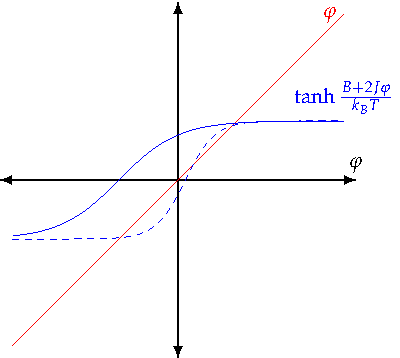
\includegraphics{Images/fig-phitranscendental.pdf}
    
    \caption{Plot of the LHS (red) and RHS (blue - solid line with $\frac{B}{k_BT} = \frac{2J}{k_BT} = 1$) of Eq. \eqref{eq-phitranscendental} as a function of $\phi$. There always exists one solution to the transcendental equation, and depending on $B$, there may exist 3 solutions (blue - dashed line with $\frac{B}{k_BT} = -\frac{1}{4}, \frac{2J}{k_BT} = 2$).}
    \label{fig-phitranscendental}
\end{figure}

It should be clear from the graph and the behavior of $\tanh$ at $\pm \infty$ (going to $\pm 1$) that we are guaranteed to have at least one solution to this expression (note that for a smaller range of $B$s, it is also possible to have three solutions). If we only have one solution, it is easy to determine which is the minimum. If we have three, we have to decide between the three; but the minimum will still be the furthest to the right (except in the case when $B = 0$, in which case the leftmost and rightmost solutions are degenerate).

Note that if we take the second derivative and plug in our solution at the minimum, we get the curvature at the minimum:
\begin{equation}
    \frac{2J}{k_B T} - \left(\frac{2J}{k_B T}\right)^2 + \left(\frac{2J}{k_B T}\right)^2\tanh^2\frac{B + 2J\phi}{k_B T}
\end{equation}
So, if the temperature is large enough, that is, $\frac{2J}{k_B T} - \left(\frac{2J}{k_B T}\right)^2$ is always positive, since the $\tanh^2$ term is always positive the second derivative of the function is always positive. So, the function is convex, and there exists one unique minimum. Specifically, this occurs when 
\begin{equation}
    T > \frac{2J}{k_B} = T_c.
\end{equation}
Conversely, when $T < T_c$ the first term can fluctuate between being positive and negative and we get two minima (Mexican hat).

\begin{figure}[htbp]
    \centering
    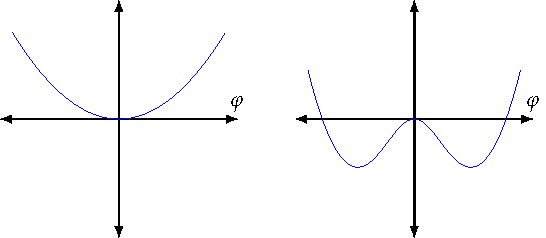
\includegraphics{Images/fig-infIsingphasetrans.pdf}


    \caption{Plot of $\frac{J\phi^2}{k_B T} - \ln\cosh\frac{B + 2J\phi}{k_B T}$ in the cases where $T > T_c$ (left - with $B = 0$ and $\frac{J}{k_B T} = \frac{1}{5}$) and $T < T_c$ (right - with $B = 0$ and $\frac{J}{k_BT} = 1$). I made a desmos graph \href{https://www.desmos.com/calculator/5d74tk33yd}{here} where you can play with $J, B$ and see how this changes the function.}
    \label{fig-infIsingphasetrans}
\end{figure}

This tells us that something ``happens'' at $T = T_c$ (specifically, a phase transition)! Note if we set $B = 0$, then the Hamiltonian has higher symmetry $\ZZ_2$; the Hamiltonian is unchanged under spin flips. So in this case the magnetization goes to zero (which we will see shortly can be identified with $\phi$). And we can also show mathematically that if $B = 0$ then the magnetization goes to zero. But if $B \neq 0$ we can have $T < T_c$, in which case $\phi = 0$ is actually a local maximum. So if $T < T_c$ we see ferromagnetism; spontaneous magnetization occurs due to the turning on of a magnetic field and a decrease in temperature.

Sketching the phase diagram for the infinite range Ising model, we have a significant difference to the standard $D = 1$ Ising model; the first phase transition persists at finite temperature at $B = 0$ (where we have the crossover of magnetization, as we go from one minimum of finite magnetization to the other (with opposite sign)). At $T = T_c$, the two minima solutions merge; they don't dissapear (really), but they go off into the complex plane where we don't have to worry about them anymore, and the $B = 0$ maxima becomes the minimum. We will see in a few moments that this is a second order phase transition!

\begin{figure}[htbp]
    \centering
    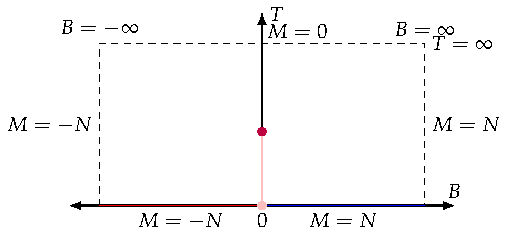
\includegraphics{Images/fig-IsingphasediagramB0.pdf}
    
    \caption{Sketch of the phase diagram of the infinite range Ising model. The first order phase transition at $B = 0$ persists at finite temperature, and at the critical temperature $T = T_c$ we have a second order phase transition.}
    \label{fig-infIsingphasediagram}
\end{figure}

For a second order phase transition, the free energy is smoother at the transition point; the first derivative exists.

\subsection{Analysis Near the Critical Temperature}
Can we be a little more analytic here? It's not so simple as we have these awful functions we are trying to minimize. If $\frac{B}{k_B T}$ is ``small'' and $T \sim T_c$ then $\phi$ is also small. Then, we are able to approximate these formulas by Taylor expanding in $\phi$ and $B$. An approximate form of the free energy reads:
\begin{equation}
    F[T, B, N] = Nk_B T \inf_\phi \left[\frac{J\phi^2}{k_B T} - \frac{1}{2}\left(\frac{2J\phi}{k_B T}\right)^2 + \frac{1}{12}\left(\frac{2J\phi + B}{k_B T}\right)^4 + \ldots \right] - k_B T N \ln 2 
\end{equation}
where we have used $\ln\cosh x = \frac{x^2}{2} + \frac{x^4}{12} + O(x^6)$. Let's analyze this expression when $B = 0$:
\begin{equation}
    F[T, B = 0, N] = -N\inf_\phi \left[J\left(1 - \frac{T_c}{T}\right)\phi^2 + \frac{1}{12}\left(\frac{T_c}{T}\right)^4\phi^4 + \ldots \right]
\end{equation}
where we have absorbed $\frac{1}{k_B T}$ into the expression inside of the infinum and used that $T_c = \frac{2J}{k_B}$.
When $T > T_c$, the solution is easily read off as $\phi = 0$. When $T < T_c$, things are a bit trickier; taking a derivative by $\phi^2$ and setting things to zero we get:
\begin{equation}
    \frac{J}{k_B T}\left(1 - \frac{T_c}{T}\right) + \frac{1}{6}\left(\frac{T_c}{T}\right)^4 \phi^2 = 0
\end{equation}
so then:
\begin{equation}
    \phi = \pm \sqrt{K\left(-1 + \frac{T_c}{T}\right)}
\end{equation}
where $K$ is some number. The free energy is then:
\begin{equation}
    F = \begin{cases}
        C & T > T_c
        \\ C + K\left(\frac{T_c}{T} - 1\right)^2 & T < T_c
    \end{cases}
\end{equation}
What we are really interested in here is how many derivatives we can take here before things go awry. It is clearly 2; when we take the first derivative, things are still continuous at $T_c$ where $F' = 0$. Taking two derivatives, we find that this is no longer continuous where at $T_c$ there is a jump from $F'' = 0$ to $F''$ some positive nonzero constant.

\subsection{Magnetization and Critical Exponents}
Now, let's try to interpret $\phi$ physically. It turns out to be the magnetization. One can argue this from the initial expression, or by calculating the magnetization explicitly:
\begin{equation}
    M = \left.-\dpd{F}{B}\right|_{T, N} = N\tanh \frac{2J\phi + B}{k_B T} = N\phi
\end{equation}
where we have used Eq. \eqref{eq-phitranscendental} in the last equality. From this we conclude:
\begin{equation}
    m = \frac{M}{N} = \phi.
\end{equation}
So all of our analysis of $\phi$ was indeed an analysis of a physical quantity. 

Another thing we can do is to set $T_c$ and approach the phase transition by varying $B$. We note that:
\begin{equation}
    m(T = T_c) \sim B^{1/3}
\end{equation}
\begin{equation}
    m(B = 0) \sim (T_c - T)^{1/2} \quad T < T_c
\end{equation}
\begin{equation}
    F \sim (T_c - T)^2 \quad T < T_c
\end{equation}
what we are interested in is the scaling behavior of $T$; these are known as critical exponents. Specifically here we are finding the critical exponents of mean field theory. This is quite profound; if a transition is described by mean field theory, they have the same critical exponents. Phase transitions with the same critical exponents have the same universality class. This was realized by Landau, who formalized the Landau theory of phase transitions. There is not much missing here from the Landau theory; the only thing which was missing is the correlation length of the system (which makes no sense for the infinite range Ising model, anyway). Note that (for systems where it is meaningful to discuss correlation lengths) the correlation lengths diverge at the phase transition, and the way these diverge are of interest indeed.

Note that it was unclear as to whether Landau theory was correct or wrong for a while; however when the 2D Ising model was solved, it was found to not have the same critical exponents as the Landau prediction (note that this does not mean that Landau theory is incorrect, only that 2D Ising lies in a different universality class. Note that for $D > 4$, Ising models are in fact well described by Landau theory/mean field theory).

Let us consider some parameters/quantities that are of interest to study when we consider phase transitions. We call $\boxed{m}$ the \emph{order parameter} in the Landau framework; the expectation value of the magnetization (per spin) tells us about the symmetry of the system (and, here, the fact that the $\ZZ_2$ symmetry is spontaneously broken at $B = 0$). We also have the (normalized) distance $\boxed{\tau}$ from the critical temperature:
\begin{equation}
    \tau = \frac{T - T_c}{T_c}
\end{equation}
We have the magnetic field $\boxed{B}$. We have the susceptibility $\boxed{\chi}$ which is:
\begin{equation}
    \chi \sim \dpd{m}{B}
\end{equation}
i.e. if we vary the field, how does the magnetization change. At the critical point, this tends to diverge. We also have the correlation length $\boxed{\xi}$ which is given by:
\begin{equation}
    \avg{\sigma_x \sigma_y} \sim e^{-\frac{1}{\xi}\abs{x - y}}
\end{equation}
where $\boxed{\avg{\sigma_x \sigma_y}}$ is a correlation function. If we drop down from the infinite range model to the standard Ising model, another parameter to consider is the dimension of the model $\boxed{D}$. We also have the specific heat $\boxed{C}$:
\begin{equation}
    C \sim \frac{T}{N}\dpd{^2F}{T^2}
\end{equation} 
We also have critical exponents (a whole family of them...). For above the phase transition $\tau > 0$, we have:
\begin{equation}
    C \sim \tau^{-\alpha}
\end{equation}
\begin{equation}
    \tau \sim \tau^{-\gamma}
\end{equation}
\begin{equation}
    \xi \sim \tau^{-\nu}
\end{equation}
below the phase transition $\tau < 0$ we have the same idea, but we put a prime on things to distinguish:
\begin{equation}
    C \sim \tau^{-\alpha'}
\end{equation}
\begin{equation}
    \tau \sim \tau^{-\gamma'}
\end{equation}
\begin{equation}
    \xi \sim \tau^{-\nu'}
\end{equation}
We also have that the order parameter scaling as:
\begin{equation}
    m \sim \tau^{\beta}
\end{equation}
for $\tau = 0, B = 0$, we have:
\begin{equation}
    B \sim m^\delta
\end{equation}
\begin{equation}
    \avg{\sigma_x\sigma_y} \sim \frac{1}{\abs{x - y}^{-d + 2 - \eta}}
\end{equation}

What we have found through our analysis is a bunch of these critical exponents. Mean field theory makes the following predictions:
\begin{equation}
    \alpha = \alpha' = 0
\end{equation}
\begin{equation}
    \beta = \frac{1}{2}
\end{equation}
\begin{equation}
    \gamma = \nu' = 1
\end{equation}
\begin{equation}
    \delta = 3
\end{equation}
We don't learn things about the correlation lengths from this model as the interactions are infinite range; but this can be fixed up via Landau-Ginsberg theory, which tells us:
\begin{equation}
    \eta = 0
\end{equation}
\begin{equation}
    \nu = \frac{1}{2}
\end{equation}
Experimental values for comparison can be compared with the table posted on the course webpage. These are not that easy to measure because they involve the scaling of something at a critical point. But some can be measured; for example $\alpha$ for the $\lambda$-transition (Bose condensation transition) in liquid Helium-4 is experimentally determined to be:
\begin{equation}
    \alpha = -0.0127 \pm 0.0003
\end{equation}
so it is known to be nonzero. So mean field theory does not quite describe this transition, though it comes close. In the theory, $\alpha = 0$ as $F \sim T^2$ and hence specific heat is a constant.